% Cover letter: Product Owner (remote, AI/data products; company not named in the posting)
% CV: Sections/cv_product_owner_data.tex -> cv_gen/2026-10-24_product_owner/cv_giovanni_tauro-product_owner.pdf
\documentclass[11pt,a4paper,sans]{moderncv}
% Shared preamble and header for the cover letters.
% One main file per application: cl_<company>.tex, built to
% cv_gen/coverletter_giovanni_tauro-<company>.pdf next to cv_giovanni_tauro-<company>.pdf.
% Paths (cl_gen/..., Pictures/...) are relative to the project root, as in the CV (see .latexmkrc).

\moderncvstyle{classic}
\moderncvcolor{blue}

\usepackage[scale=0.80]{geometry}
\setlength{\footskip}{136.00005pt}

\usepackage{fontawesome5}
% hyperref is loaded by moderncv itself; loading it here causes an option clash
\usepackage{xcolor}
\usepackage{graphicx}
\ifxetexorluatex
  \usepackage{fontspec}
  \usepackage{unicode-math}
  \defaultfontfeatures{Ligatures=TeX}
  \setmainfont{Latin Modern Roman}
  \setsansfont{Latin Modern Sans}
  \setmonofont{Latin Modern Mono}
  \setmathfont{Latin Modern Math}
\else
  \usepackage[T1]{fontenc}
  \usepackage{lmodern}
\fi

\usepackage[english]{babel}

% used for the PDF title and the letter closing; the visible header is \clheader below
\name{Giovanni}{Tauro}

% Header: #1 = headline under the name (same as the headline of the matching CV)
\newcommand{\clheader}[1]{%
\noindent
\begin{minipage}[c]{0.74\textwidth}
    {\Huge \textbf{Giovanni Tauro}}\\[-0.2em]
    {\small #1}\\[0.3em]

    \footnotesize
    \faMapMarker*~
    \href{https://www.google.com/maps/search/?api=1&query=Lecco+23900+Italy}
    {\color{blue}Bari-Lecco, Italy}
    \quad
    \faPhone*~
    \href{https://wa.me/393279437161}
    {\color{blue}+39 3279437161}
    \quad
    \faEnvelope~
    \href{mailto:giovanni.taurodi@gmail.com}
    {\color{blue}giovanni.taurodi@gmail.com}
    \\[-0.1em]

    \faLinkedin~
    \href{https://www.linkedin.com/in/giovanni-tauro-gt/}
    {\color{blue}LinkedIn}
    \quad
    \faGithub~
    \href{https://github.com/jotades}
    {\color{blue}GitHub}
    \quad
    \faGraduationCap~
    \href{https://scholar.google.com/citations?user=BS0aVGgAAAAJ&hl=it}
    {\color{blue}Scholar}
    \quad
    \faFilePdf~
    \href{https://www.notion.so/Giovanni-Tauro-2a7901d92f3a800b892af425c5875c6a}
    {\color{blue}Portfolio}
    \quad
    \faCubes~
    \href{https://grabcad.com/giovanni.tauro-3}
    {\color{blue}GrabCAD}

\end{minipage}
\hfill
\begin{minipage}[c]{0.18\textwidth}
    \raggedleft
    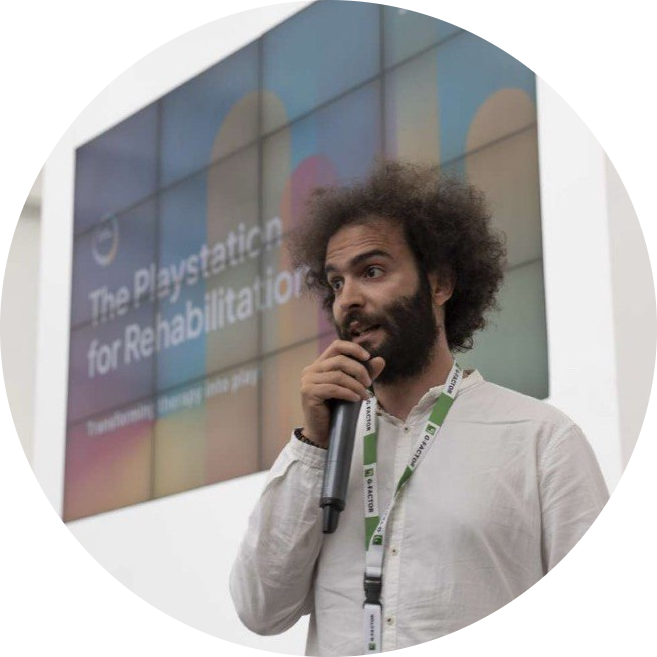
\includegraphics[width=2.8cm]{Pictures/Giovanni_pitch}
\end{minipage}
\vspace{0.1em}
}

\makeatletter
% the sender details are already in \clheader, so skip moderncv's own block
\@detailsfalse
% closing phrase, signature, name
\renewcommand*{\makeletterclosing}{%
  \@closing\\[0.6em]%
  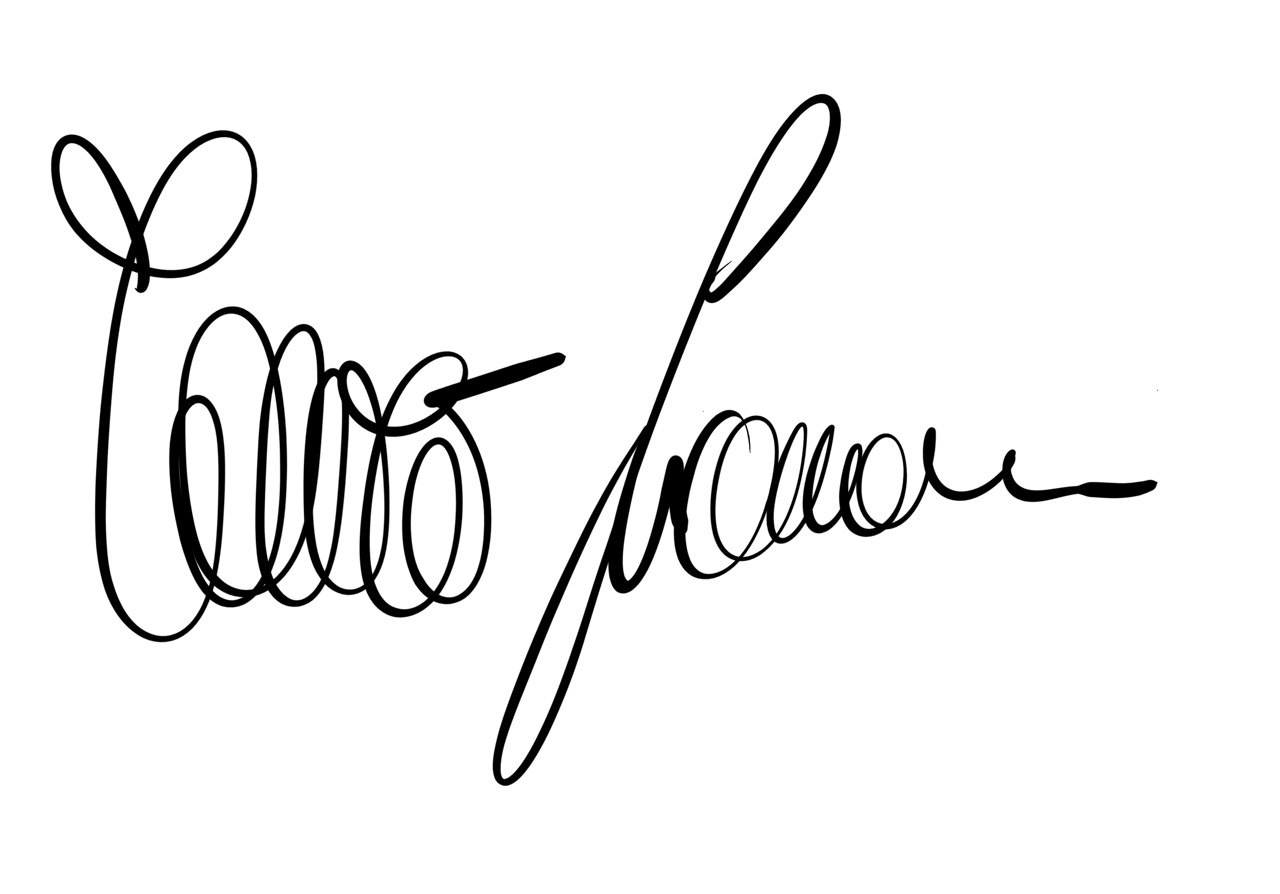
\includegraphics[height=1.2cm]{Pictures/sign_gt.jpg}\\[0.2em]%
  {\bfseries\@firstname~\@lastname}}
\makeatother


\begin{document}

\clheader{Product Owner | Discovery, UX \& Data Products}

\recipient{Hiring Team}{Product Owner (Remote)}
\opening{Dear Hiring Team,}
\closing{Sincerely,}
\makelettertitle

I am applying for the Product Owner role. I am Head of Product and co-founder of Rehabilia Technologies, and for more than five years I have built products for expert users at CNR-STIIMA, the Italian National Research Council. You are looking for someone who turns complex problems into products people enjoy using, in close partnership with engineering and data teams; that is the core of my work.

At Rehabilia I own the product from discovery to release. I interview clinicians, patients and partners, frame the problem, write the requirements and prioritise a backlog that is always larger than capacity, using study data and user feedback to decide what enters each release and to explain what waits. Our device, PhiCube, went from user research and prototypes to clinical use: it reached a usability score of 85.8/100 (SUS) with 19 children and is now in two ongoing multicentre studies with 134 patients. Preliminary results from six Italian clinics are encouraging: 55 children aged 4 to 17 rated every usability and acceptability item above 4 out of 5, and 70\% experienced it as a game rather than therapy, which is what keeps them engaged. Getting there meant aligning engineers, clinicians, research partners and funders on the same trade-offs.

I am at ease with technically complex products. For my PhD project, OmniTrack, an indoor navigation system for blind users, I designed OmniAnalytics, a data tool that turns raw session recordings from 16 participants into trial metrics, with correction flows that never alter the raw records. I analyse data in Python, work closely with engineers on data flows and system design, and co-authored research on socially interactive AI agents for rehabilitation. I use Claude and Claude Code every day to prototype ideas and analyse data, and I hold Anthropic's certifications for both.

My products so far have been a medical device with its software and research tools rather than a commercial SaaS with a large user base, so I have measured outcomes mainly through usability scores, study data and user feedback rather than adoption funnels. What I bring is the habit of asking which outcome a release should change before it is built, and checking it with real users afterwards.

I would welcome the chance to discuss the role further.

\makeletterclosing

\end{document}
